\chapter{Colorization}
\label{chapterlabel3}

Colorization is the process of adding plausible colors to monochrome images, it is a highly uncertain problem that has not a unique solution. In the context of this master project, we are interested in anime-style sketch colorization, a few distinctive characteristics includes:

\begin{itemize}
    \item Unlike grayscale image input, its input is a binary sketch image.
    \item Unlike realistic image colorization, the output is heavily style-oriented, has less well-defined boundaries, and therefore a more nondeterministic nature.
    \item Unlike many colorization papers, the task of filling cropped region is not assessed. The full sketch image is provided without cropping.
    \item It is relatively difficult to find a dataset that contains large amount of high quality pairs of sketch and colorized anime image, because artists often does not include it when uploading to the internet.
\end{itemize}


\section{Approaches \& Methods}
Anime-style sketch colorization is a difficult problem because there are infinite number of ways to produce feasible results, therefore color strokes are often given as additional input to hint the model to output in a certain style. There are many attempts to this problem and I will introduce them in the following paragraphs.

Traditional computer assisted colorization uses an algorithmic approach. Typically, the user first crops the region that he/she wants to color, then apply a color scheme from a palette, finally the computer will run an algorithm to perform colorization. A popular approach is to minimize the difference between a pixel's color and its weighted average of neighbouring pixels' colors.\cite{levinColorizationUsingOptimizationb} The intuitive is neighboring pixels with similar intensity should have similar colors. This method generates high quality results, but it is time consuming, additionally, anime sketches are often binary and does not include intensity information, therefore it is not suitable.



\begin{figure}
    \centering
    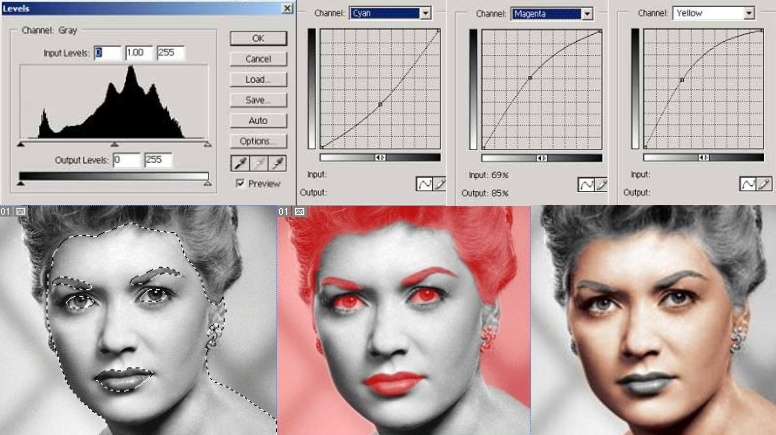
\includegraphics[width=0.75\textwidth]{images/colorization/computer_assisted_colorization.jpg}
    \caption{Example interface for traditional computer assisted algorithmic colorization. Top shows an interface for selecting a color; bottom-left and bottom-middle show interfaces for selecting a region; and bottom-right shows the resulting image.\cite{ColorizeBlackWhite}}
    \label{fig:computer_assisted_colorization}
\end{figure}

\section{Design \& Implementation}
\section{Results \& Analysis}
% This just dumps some pseudolatin in so you can see some text in place.
\blindtext
